\documentclass{standalone}
\usepackage{tikz}
\usetikzlibrary{patterns, positioning}


\begin{document}
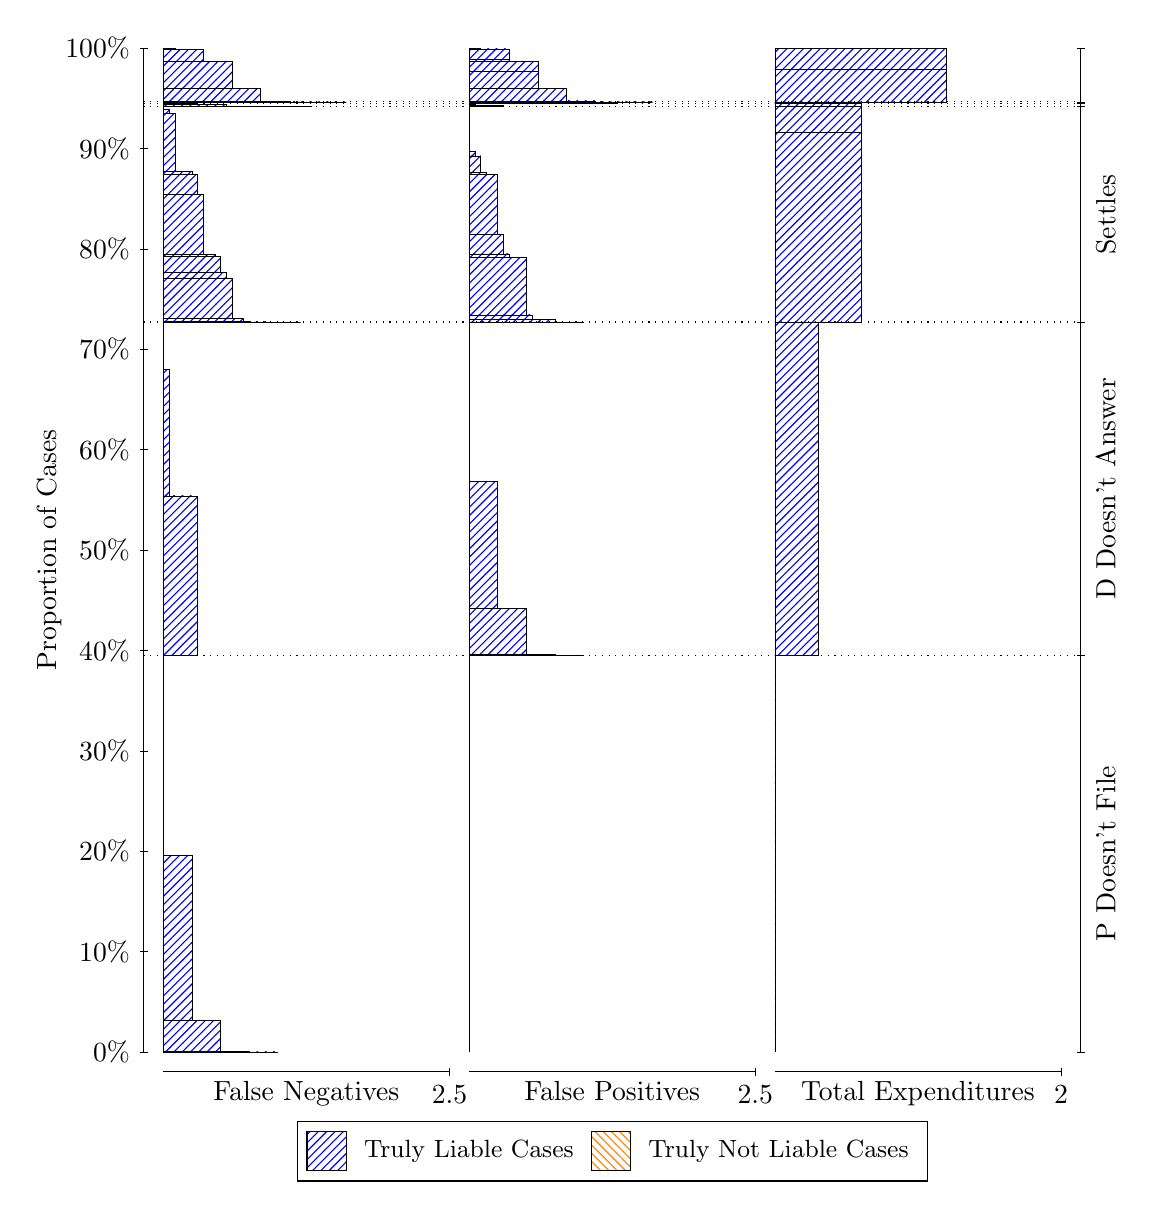
\begin{tikzpicture}
\draw[black, very thin] (1.5,1.75) -- (1.5,14.5);
\node[rotate=90, text=black, anchor=center] at (0.3, 8.125) {Proportion of Cases};
\draw[black, very thin] (1.45,1.75) -- (1.55,1.75);
\node[text=black, anchor=east] at (1.45, 1.75) {0\%};
\draw[black, very thin] (1.45,3.025) -- (1.55,3.025);
\node[text=black, anchor=east] at (1.45, 3.025) {10\%};
\draw[black, very thin] (1.45,4.3) -- (1.55,4.3);
\node[text=black, anchor=east] at (1.45, 4.3) {20\%};
\draw[black, very thin] (1.45,5.575) -- (1.55,5.575);
\node[text=black, anchor=east] at (1.45, 5.575) {30\%};
\draw[black, very thin] (1.45,6.85) -- (1.55,6.85);
\node[text=black, anchor=east] at (1.45, 6.85) {40\%};
\draw[black, very thin] (1.45,8.125) -- (1.55,8.125);
\node[text=black, anchor=east] at (1.45, 8.125) {50\%};
\draw[black, very thin] (1.45,9.4) -- (1.55,9.4);
\node[text=black, anchor=east] at (1.45, 9.4) {60\%};
\draw[black, very thin] (1.45,10.675) -- (1.55,10.675);
\node[text=black, anchor=east] at (1.45, 10.675) {70\%};
\draw[black, very thin] (1.45,11.95) -- (1.55,11.95);
\node[text=black, anchor=east] at (1.45, 11.95) {80\%};
\draw[black, very thin] (1.45,13.225) -- (1.55,13.225);
\node[text=black, anchor=east] at (1.45, 13.225) {90\%};
\draw[black, very thin] (1.45,14.5) -- (1.55,14.5);
\node[text=black, anchor=east] at (1.45, 14.5) {100\%};

\draw[black, very thin] (13.4,1.75) -- (13.4,14.5);
\draw[black, very thin] (13.35,1.75) -- (13.45,1.75);
\node[anchor=west] at (13.35, 1.75) {};
\draw[black, very thin] (13.35,6.7852) -- (13.45,6.7852);
\node[anchor=west] at (13.35, 6.7852) {};
\draw[black, very thin] (13.35,11.02) -- (13.45,11.02);
\node[anchor=west] at (13.35, 11.02) {};
\draw[black, very thin] (13.35,13.757) -- (13.45,13.757);
\node[anchor=west] at (13.35, 13.757) {};
\draw[black, very thin] (13.35,13.792) -- (13.45,13.792);
\node[anchor=west] at (13.35, 13.792) {};
\draw[black, very thin] (13.35,13.816) -- (13.45,13.816);
\node[anchor=west] at (13.35, 13.816) {};
\draw[black, very thin] (13.35,14.5) -- (13.45,14.5);
\node[anchor=west] at (13.35, 14.5) {};

\draw[black, very thin, pattern color=blue, pattern=north east lines] (1.75,1.75) rectangle (3.2033,1.75);
\draw[black, very thin, pattern color=blue, pattern=north east lines] (1.75,1.75) rectangle (2.84,1.7534);
\draw[black, very thin, pattern color=blue, pattern=north east lines] (1.75,1.7534) rectangle (2.4767,2.1482);
\draw[black, very thin, pattern color=blue, pattern=north east lines] (1.75,2.1482) rectangle (2.1133,4.2508);
\draw[black, very thin, pattern color=orange, pattern=north west lines] (1.75,4.2508) rectangle (1.75,4.2508);
\draw[black, very thin, pattern color=blue, pattern=north east lines] (1.75,4.2508) rectangle (1.75,6.7852);
\draw[black, very thin, pattern color=blue, pattern=north east lines] (1.75,6.7852) rectangle (2.186,8.8114);
\draw[black, very thin, pattern color=blue, pattern=north east lines] (1.75,8.8114) rectangle (1.8227,10.418);
\draw[black, very thin, pattern color=orange, pattern=north west lines] (1.75,10.418) rectangle (1.75,10.418);
\draw[black, very thin, pattern color=blue, pattern=north east lines] (1.75,10.418) rectangle (1.75,11.02);
\draw[black, very thin, pattern color=blue, pattern=north east lines] (1.75,11.02) rectangle (3.494,11.02);
\draw[black, very thin, pattern color=blue, pattern=north east lines] (1.75,11.02) rectangle (3.2033,11.02);
\draw[black, very thin, pattern color=blue, pattern=north east lines] (1.75,11.02) rectangle (3.1307,11.021);
\draw[black, very thin, pattern color=blue, pattern=north east lines] (1.75,11.021) rectangle (2.9127,11.023);
\draw[black, very thin, pattern color=blue, pattern=north east lines] (1.75,11.023) rectangle (2.84,11.032);
\draw[black, very thin, pattern color=blue, pattern=north east lines] (1.75,11.032) rectangle (2.7673,11.071);
\draw[black, very thin, pattern color=blue, pattern=north east lines] (1.75,11.071) rectangle (2.622,11.582);
\draw[black, very thin, pattern color=blue, pattern=north east lines] (1.75,11.582) rectangle (2.5493,11.647);
\draw[black, very thin, pattern color=blue, pattern=north east lines] (1.75,11.647) rectangle (2.4767,11.854);
\draw[black, very thin, pattern color=blue, pattern=north east lines] (1.75,11.854) rectangle (2.404,11.883);
\draw[black, very thin, pattern color=blue, pattern=north east lines] (1.75,11.883) rectangle (2.2587,12.646);
\draw[black, very thin, pattern color=blue, pattern=north east lines] (1.75,12.646) rectangle (2.186,12.891);
\draw[black, very thin, pattern color=blue, pattern=north east lines] (1.75,12.891) rectangle (2.1133,12.937);
\draw[black, very thin, pattern color=blue, pattern=north east lines] (1.75,12.937) rectangle (2.0407,12.937);
\draw[black, very thin, pattern color=blue, pattern=north east lines] (1.75,12.937) rectangle (1.8953,13.666);
\draw[black, very thin, pattern color=blue, pattern=north east lines] (1.75,13.666) rectangle (1.8227,13.728);
\draw[black, very thin, pattern color=orange, pattern=north west lines] (1.75,13.728) rectangle (1.75,13.728);
\draw[black, very thin, pattern color=blue, pattern=north east lines] (1.75,13.728) rectangle (1.75,13.757);
\draw[black, very thin, pattern color=blue, pattern=north east lines] (1.75,13.757) rectangle (3.6393,13.757);
\draw[black, very thin, pattern color=blue, pattern=north east lines] (1.75,13.757) rectangle (3.276,13.757);
\draw[black, very thin, pattern color=blue, pattern=north east lines] (1.75,13.757) rectangle (2.9127,13.759);
\draw[black, very thin, pattern color=blue, pattern=north east lines] (1.75,13.759) rectangle (2.5493,13.781);
\draw[black, very thin, pattern color=blue, pattern=north east lines] (1.75,13.781) rectangle (2.186,13.792);
\draw[black, very thin, pattern color=orange, pattern=north west lines] (1.75,13.792) rectangle (1.75,13.792);
\draw[black, very thin, pattern color=blue, pattern=north east lines] (1.75,13.792) rectangle (2.186,13.802);
\draw[black, very thin, pattern color=blue, pattern=north east lines] (1.75,13.802) rectangle (1.8227,13.816);
\draw[black, very thin, pattern color=orange, pattern=north west lines] (1.75,13.816) rectangle (1.75,13.816);
\draw[black, very thin, pattern color=blue, pattern=north east lines] (1.75,13.816) rectangle (1.75,13.816);
\draw[black, very thin, pattern color=blue, pattern=north east lines] (1.75,13.816) rectangle (4.0753,13.816);
\draw[black, very thin, pattern color=blue, pattern=north east lines] (1.75,13.816) rectangle (3.712,13.816);
\draw[black, very thin, pattern color=blue, pattern=north east lines] (1.75,13.816) rectangle (3.3487,13.826);
\draw[black, very thin, pattern color=blue, pattern=north east lines] (1.75,13.826) rectangle (2.9853,13.984);
\draw[black, very thin, pattern color=blue, pattern=north east lines] (1.75,13.984) rectangle (2.622,14.328);
\draw[black, very thin, pattern color=blue, pattern=north east lines] (1.75,14.328) rectangle (2.2587,14.486);
\draw[black, very thin, pattern color=blue, pattern=north east lines] (1.75,14.486) rectangle (1.8953,14.5);
\draw[black, very thin, pattern color=orange, pattern=north west lines] (1.75,14.5) rectangle (1.75,14.5);
\draw[black, very thin, pattern color=blue, pattern=north east lines] (1.75,14.5) rectangle (1.75,14.5);
\draw[black, very thin, pattern color=orange, pattern=north west lines] (5.6333,1.75) rectangle (5.6333,1.75);
\draw[black, very thin, pattern color=blue, pattern=north east lines] (5.6333,1.75) rectangle (5.6333,6.7852);
\draw[black, very thin, pattern color=orange, pattern=north west lines] (5.6333,6.7852) rectangle (7.0867,6.7852);
\draw[black, very thin, pattern color=blue, pattern=north east lines] (5.6333,6.7852) rectangle (7.0867,6.7852);
\draw[black, very thin, pattern color=blue, pattern=north east lines] (5.6333,6.7852) rectangle (6.7233,6.801);
\draw[black, very thin, pattern color=blue, pattern=north east lines] (5.6333,6.801) rectangle (6.36,7.3876);
\draw[black, very thin, pattern color=blue, pattern=north east lines] (5.6333,7.3876) rectangle (5.9967,8.9938);
\draw[black, very thin, pattern color=blue, pattern=north east lines] (5.6333,8.9938) rectangle (5.6333,11.02);
\draw[black, very thin, pattern color=orange, pattern=north west lines] (5.6333,11.02) rectangle (7.0867,11.02);
\draw[black, very thin, pattern color=blue, pattern=north east lines] (5.6333,11.02) rectangle (7.0867,11.02);
\draw[black, very thin, pattern color=orange, pattern=north west lines] (5.6333,11.02) rectangle (6.796,11.02);
\draw[black, very thin, pattern color=blue, pattern=north east lines] (5.6333,11.02) rectangle (6.796,11.022);
\draw[black, very thin, pattern color=blue, pattern=north east lines] (5.6333,11.022) rectangle (6.7233,11.049);
\draw[black, very thin, pattern color=orange, pattern=north west lines] (5.6333,11.049) rectangle (6.5053,11.049);
\draw[black, very thin, pattern color=blue, pattern=north east lines] (5.6333,11.049) rectangle (6.5053,11.049);
\draw[black, very thin, pattern color=blue, pattern=north east lines] (5.6333,11.049) rectangle (6.4327,11.111);
\draw[black, very thin, pattern color=blue, pattern=north east lines] (5.6333,11.111) rectangle (6.36,11.84);
\draw[black, very thin, pattern color=orange, pattern=north west lines] (5.6333,11.84) rectangle (6.2147,11.84);
\draw[black, very thin, pattern color=blue, pattern=north east lines] (5.6333,11.84) rectangle (6.2147,11.84);
\draw[black, very thin, pattern color=blue, pattern=north east lines] (5.6333,11.84) rectangle (6.142,11.886);
\draw[black, very thin, pattern color=blue, pattern=north east lines] (5.6333,11.886) rectangle (6.0693,12.13);
\draw[black, very thin, pattern color=blue, pattern=north east lines] (5.6333,12.13) rectangle (5.9967,12.893);
\draw[black, very thin, pattern color=blue, pattern=north east lines] (5.6333,12.893) rectangle (5.8513,12.923);
\draw[black, very thin, pattern color=blue, pattern=north east lines] (5.6333,12.923) rectangle (5.7787,13.13);
\draw[black, very thin, pattern color=blue, pattern=north east lines] (5.6333,13.13) rectangle (5.706,13.195);
\draw[black, very thin, pattern color=blue, pattern=north east lines] (5.6333,13.195) rectangle (5.6333,13.757);
\draw[black, very thin, pattern color=orange, pattern=north west lines] (5.6333,13.757) rectangle (6.0693,13.757);
\draw[black, very thin, pattern color=blue, pattern=north east lines] (5.6333,13.757) rectangle (6.0693,13.767);
\draw[black, very thin, pattern color=blue, pattern=north east lines] (5.6333,13.767) rectangle (5.706,13.79);
\draw[black, very thin, pattern color=blue, pattern=north east lines] (5.6333,13.79) rectangle (5.6333,13.792);
\draw[black, very thin, pattern color=orange, pattern=north west lines] (5.6333,13.792) rectangle (7.5227,13.792);
\draw[black, very thin, pattern color=blue, pattern=north east lines] (5.6333,13.792) rectangle (7.5227,13.792);
\draw[black, very thin, pattern color=blue, pattern=north east lines] (5.6333,13.792) rectangle (7.1593,13.792);
\draw[black, very thin, pattern color=blue, pattern=north east lines] (5.6333,13.792) rectangle (6.796,13.792);
\draw[black, very thin, pattern color=blue, pattern=north east lines] (5.6333,13.792) rectangle (6.4327,13.807);
\draw[black, very thin, pattern color=blue, pattern=north east lines] (5.6333,13.807) rectangle (6.0693,13.816);
\draw[black, very thin, pattern color=orange, pattern=north west lines] (5.6333,13.816) rectangle (7.9587,13.816);
\draw[black, very thin, pattern color=blue, pattern=north east lines] (5.6333,13.816) rectangle (7.9587,13.816);
\draw[black, very thin, pattern color=orange, pattern=north west lines] (5.6333,13.816) rectangle (7.5953,13.816);
\draw[black, very thin, pattern color=blue, pattern=north east lines] (5.6333,13.816) rectangle (7.5953,13.817);
\draw[black, very thin, pattern color=orange, pattern=north west lines] (5.6333,13.817) rectangle (7.232,13.817);
\draw[black, very thin, pattern color=blue, pattern=north east lines] (5.6333,13.817) rectangle (7.232,13.83);
\draw[black, very thin, pattern color=blue, pattern=north east lines] (5.6333,13.83) rectangle (6.8687,13.988);
\draw[black, very thin, pattern color=orange, pattern=north west lines] (5.6333,13.988) rectangle (6.8687,13.988);
\draw[black, very thin, pattern color=blue, pattern=north east lines] (5.6333,13.988) rectangle (6.8687,13.989);
\draw[black, very thin, pattern color=blue, pattern=north east lines] (5.6333,13.989) rectangle (6.5053,14.206);
\draw[black, very thin, pattern color=orange, pattern=north west lines] (5.6333,14.206) rectangle (6.5053,14.206);
\draw[black, very thin, pattern color=blue, pattern=north east lines] (5.6333,14.206) rectangle (6.5053,14.332);
\draw[black, very thin, pattern color=blue, pattern=north east lines] (5.6333,14.332) rectangle (6.142,14.353);
\draw[black, very thin, pattern color=blue, pattern=north east lines] (5.6333,14.353) rectangle (6.142,14.49);
\draw[black, very thin, pattern color=blue, pattern=north east lines] (5.6333,14.49) rectangle (5.7787,14.49);
\draw[black, very thin, pattern color=blue, pattern=north east lines] (5.6333,14.49) rectangle (5.7787,14.5);
\draw[black, very thin, pattern color=blue, pattern=north east lines] (5.6333,14.5) rectangle (5.6333,14.5);
\draw[black, very thin, pattern color=orange, pattern=north west lines] (9.5167,1.75) rectangle (9.5167,1.75);
\draw[black, very thin, pattern color=blue, pattern=north east lines] (9.5167,1.75) rectangle (9.5167,6.7852);
\draw[black, very thin, pattern color=orange, pattern=north west lines] (9.5167,6.7852) rectangle (10.062,6.7852);
\draw[black, very thin, pattern color=blue, pattern=north east lines] (9.5167,6.7852) rectangle (10.062,11.02);
\draw[black, very thin, pattern color=orange, pattern=north west lines] (9.5167,11.02) rectangle (10.607,11.02);
\draw[black, very thin, pattern color=blue, pattern=north east lines] (9.5167,11.02) rectangle (10.607,13.425);
\draw[black, very thin, pattern color=orange, pattern=north west lines] (9.5167,13.425) rectangle (10.607,13.425);
\draw[black, very thin, pattern color=blue, pattern=north east lines] (9.5167,13.425) rectangle (10.607,13.757);
\draw[black, very thin, pattern color=orange, pattern=north west lines] (9.5167,13.757) rectangle (10.607,13.757);
\draw[black, very thin, pattern color=blue, pattern=north east lines] (9.5167,13.757) rectangle (10.607,13.792);
\draw[black, very thin, pattern color=orange, pattern=north west lines] (9.5167,13.792) rectangle (10.607,13.792);
\draw[black, very thin, pattern color=blue, pattern=north east lines] (9.5167,13.792) rectangle (10.607,13.816);
\draw[black, very thin, pattern color=orange, pattern=north west lines] (9.5167,13.816) rectangle (11.697,13.816);
\draw[black, very thin, pattern color=blue, pattern=north east lines] (9.5167,13.816) rectangle (11.697,14.226);
\draw[black, very thin, pattern color=orange, pattern=north west lines] (9.5167,14.226) rectangle (11.697,14.226);
\draw[black, very thin, pattern color=blue, pattern=north east lines] (9.5167,14.226) rectangle (11.697,14.5);
\draw[black, dotted] (1.5,6.7852) -- (13.4,6.7852);
\draw[black, dotted] (1.5,11.02) -- (13.4,11.02);
\draw[black, dotted] (1.5,13.757) -- (13.4,13.757);
\draw[black, dotted] (1.5,13.792) -- (13.4,13.792);
\draw[black, dotted] (1.5,13.816) -- (13.4,13.816);
\draw[black, very thin] (1.75,1.5) -- (5.3833,1.5);
\node[text=black, anchor=north] at (3.5667, 1.5) {False Negatives};
\draw[black, very thin] (5.3833,1.45) -- (5.3833,1.55);
\node[text=black, anchor=north] at (5.3833, 1.45) {2.5};

\draw[black, very thin] (5.6333,1.5) -- (9.2667,1.5);
\node[text=black, anchor=north] at (7.45, 1.5) {False Positives};
\draw[black, very thin] (9.2667,1.45) -- (9.2667,1.55);
\node[text=black, anchor=north] at (9.2667, 1.45) {2.5};

\draw[black, very thin] (9.5167,1.5) -- (13.15,1.5);
\node[text=black, anchor=north] at (11.333, 1.5) {Total Expenditures};
\draw[black, very thin] (13.15,1.45) -- (13.15,1.55);
\node[text=black, anchor=north] at (13.15, 1.45) {2};

\node[text=black, centered, rotate=90] at (13.72, 4.2676) {P Doesn't File};
\node[text=black, centered, rotate=90] at (13.72, 8.9026) {D Doesn't Answer};
\node[text=black, centered, rotate=90] at (13.72, 12.388) {Settles};




\draw (7.449999999999999,1.5) node[draw=none] (baseCoordinate) {};
\begin{scope}[align=center]
        \matrix[scale=0.5, draw=black, below=0.5cm of baseCoordinate, nodes={draw}, column sep=0.1cm]{
            \node[rectangle, draw, minimum width=0.5cm, minimum height=0.5cm, pattern color=blue, pattern=north east lines] {}; &
            \node[draw=none, font=\small, text=black] (B) {Truly Liable Cases}; &
            \node[rectangle, draw, minimum width=0.5cm, minimum height=0.5cm, pattern color=orange, pattern=north west lines] {}; &
            \node[draw=none, font=\small, text=black] (B) {Truly Not Liable Cases}; \\
            };
\end{scope}

\end{tikzpicture}
\end{document}